\subsection{Organisation}

\textbf{Organisation}: A structured group of people working together to achieve specific goals or purposes.

\begin{itemize}
    \item \textbf{Formal}: A company, school, government agency, or non-profit.
    \item \textbf{Informal}: A community group or club.
\end{itemize}

\subsubsection{Characteristics}

\begin{itemize}
    \item \textbf{Purpose}: A mission or objective that guides its activities.
    \item \textbf{People}: Individuals with different roles, responsibilities, and skills.
    \item \textbf{Structure}: A defined hierarchy that outlines how tasks are divided and coordinated.
    \item \textbf{System} Methods for communication, decision making, and operations.
    \item \textbf{Resources} They utilize human, financial, technological, and physical resources.
\end{itemize}

\subsubsection{Organisation VS Business}

\indent

\textbf{Organisation}: a \textbf{broad term} that refers to any group of people working together in a structured way to achieve a common goal. \textbf{Not always profit-driven.}

\textbf{Business}: \textbf{a type of Organisation} whose \textbf{primary goal is to make a profit} by providing goods or services.

\begin{table}[h]
    \centering
    \begin{tabular}{c|c}
        \hline
        Organisation & Business \\\hline
        Non-profits – Red Cross & Startups – Canva\\
        Governments – NSW Health & Corporations – Apple\\
        Universities – University of Sydney & Small Businesses – Local cafes\\
        Clubs – Local sports club & \\\hline
    \end{tabular}
    \caption{Some examples}
\end{table}

\subsection{Organisational Structure}

\textbf{Organisational Structure}: 

It defines \textbf{how tasks, responsibilities, and authority are distributed} within an Organisation. 

It shows the \textbf{hierarchy, reporting lines}, and how different roles and departments \textbf{interact and coordinate} with each other.

\subsubsection{Why Organisational Structure Important?}

\begin{itemize}
    \item Clarifies who reports to whom
    \item Defines decision-making authority
    \item Improves efficiency and communication
    \item Helps manage growth and change
\end{itemize}

\subsubsection{Type of Organisational Structure}

\begin{itemize}
    \item \textbf{Functional}: Groups employees based on specialized roles or functions.
    \item \textbf{Matrix}: Employees report to two managers - one for function, one for project.
    \item \textbf{Flat}: Few or no levels of middle management. Common in startups or small Organisations.
    \item \textbf{Hierarchical}: Traditional structure with clear top-down command and multiple layers of authority.
\end{itemize}

\subsubsection{Organisational Structures - Functional}

\begin{figure}[h]
    \centering
    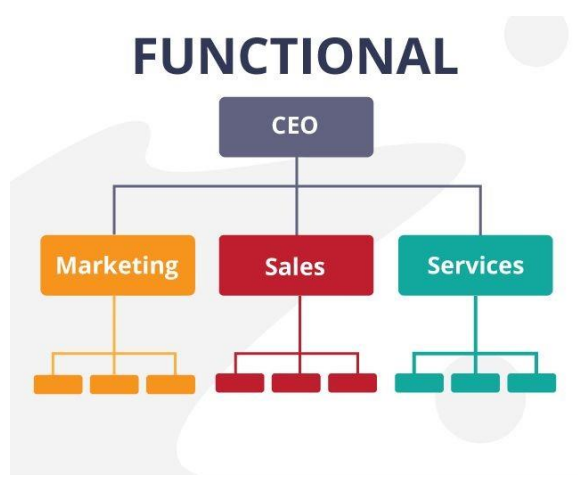
\includegraphics[width=0.5\linewidth]{figures/Week 2/Functional.png}
\end{figure}

\noindent\textbf{Functional}: Organisation is divided into departments 
based on specific functions (e.g., IT, HR, Finance, Marketing).

\noindent\textbf{Best For:} Large or growing organisations with clearly defined departments (e.g., tech companies, banks, \textbf{Microsoft}).

\bigskip

\noindent\textbf{Pros:}

\begin{itemize}
    \item Specialisation leads to efficiency
    \item Clear roles and responsibilities
    \item Easier to manage and scale by department
\end{itemize}

\bigskip

\noindent\textbf{Cons:}

\begin{itemize}
    \item Limited communication across departments
    \item Can create silos and reduce flexibility
\end{itemize}

\subsubsection{Organisational Structures - Matrix}

\begin{figure}[h]
    \centering
    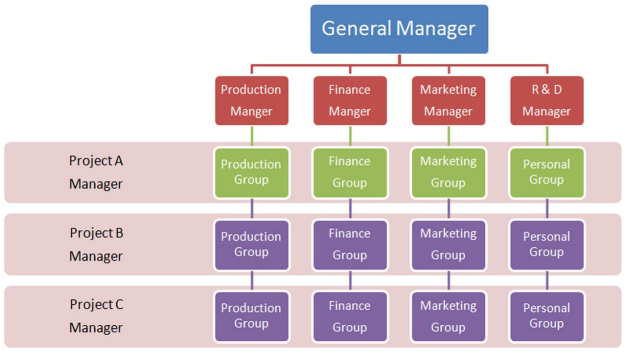
\includegraphics[width=0.8\linewidth]{figures/Week 2/Matrix.png}
\end{figure}

\noindent\textbf{Matrix}: Employees report to more than one manager, typically by function and project/team.

\noindent\textbf{Best For:} Project-based or global companies (e.g., consulting firms, R\&D, IT services companies, \textbf{Google}).

\bigskip

\noindent\textbf{Pros:}

\begin{itemize}
    \item Efficient use of resources across projects
    \item Encourages teamwork and cross functional skills
    \item Increases flexibility and adaptability
\end{itemize}

\bigskip

\noindent\textbf{Cons:}

\begin{itemize}
    \item Dual authority can cause confusion
    \item Requires strong communication and coordination
\end{itemize}

\subsubsection{Organisational Structures - Flat}

\begin{figure}[h]
    \centering
    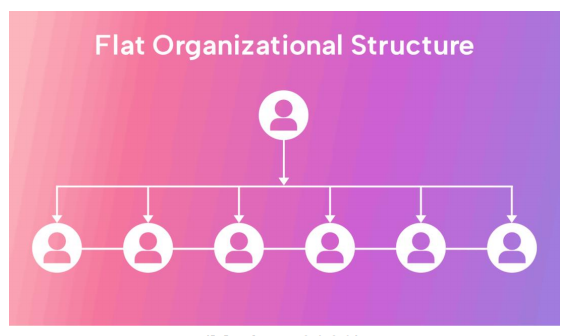
\includegraphics[width=0.5\linewidth]{figures/Week 2/Flat.png}
\end{figure}

\noindent\textbf{Flat}: Few or no levels of middle management between staff and leadership. Everyone is closer to decision-making.

\noindent\textbf{Best For:} Startups or small teams where agility and speed matter more than hierarchy. (e.g., \textbf{Valve})

\bigskip

\noindent\textbf{Pros:}

\begin{itemize}
    \item Fast communication and decision making
    \item Encourages innovation and collaboration
    \item Flexible and adaptive
\end{itemize}

\bigskip

\noindent\textbf{Cons:}

\begin{itemize}
    \item Can lead to confusion in roles/responsibilities
    \item Not scalable for large teams
\end{itemize}

\subsubsection{Organisational Structures - Hierarchical}

\begin{figure}[h]
    \centering
    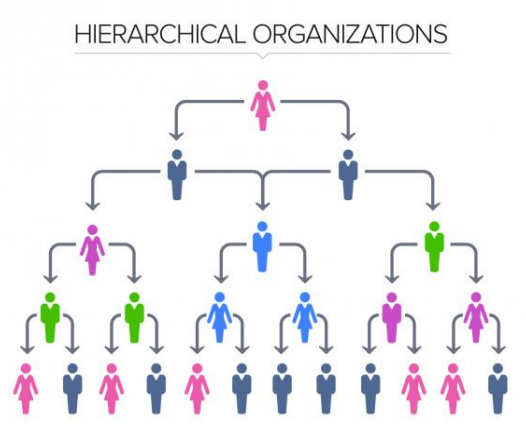
\includegraphics[width=0.5\linewidth]{figures/Week 2/Hierarchical.png}
\end{figure}

\noindent\textbf{Hierarchical}: Traditional top-down approach with multiple levels of authority and a clear chain of command.

\noindent\textbf{Best For:} Government bodies, large enterprises, 
and traditional corporations. (e.g., \textbf{IBM})

\bigskip

\noindent\textbf{Pros:}

\begin{itemize}
    \item Clear reporting lines and accountability
    \item Stable and easy to manage large teams
    \item Supports growth and delegation
\end{itemize}

\bigskip

\noindent\textbf{Cons:}

\begin{itemize}
    \item Slower decision-making
    \item Can stifle creativity and employee autonomy
\end{itemize}

\subsection{Value and Organisational Value}

\subsubsection{Value}

\textbf{Value}: refers to the \textbf{worth}, \textbf{usefulness}, or \textbf{benefit} of something.

\begin{itemize}
    \item Tangible (e.g., Money, Products)
    \item Intangible (e.g., Trust, Satisfaction)
\end{itemize}

\subsubsection{Organisational Value}

\textbf{Organisational Value}: refers to the \textbf{value created}, \textbf{delivered}, and \textbf{sustained} by an Organisation for its stakeholders, including customers, employees, shareholders, and society.

\subsubsection{Value VS Organisational Value}

% Please add the following required packages to your document preamble:
% \usepackage{multirow}
\begin{table}[h]
\begin{tabular}{|c|c|l|}
\hline
\multirow{2}{*}{Scope}        & Value                & \begin{tabular}[c]{@{}l@{}}Broad and general – can apply to anything, anyone, or any idea,\\ not limited to a business context.\end{tabular}                                    \\ \cline{2-3} 
                              & Organisational Value & \begin{tabular}[c]{@{}l@{}}Narrower and specific - relates only to what an organisation \\ creates, delivers, and sustains through its operations and mission.\end{tabular}     \\ \hline
\multirow{2}{*}{Focus}        & Value                & \begin{tabular}[c]{@{}l@{}}Centers on the worth of an individual item, idea, or experience \\ (e.g., the usefulness of a product).\end{tabular}                                 \\ \cline{2-3} 
                              & Organisational Value & \begin{tabular}[c]{@{}l@{}}Centers on the overall value an organisation, provides through \\ its products, services, operations, and impact.\end{tabular}                       \\ \hline
\multirow{2}{*}{Stakeholders} & Value                & \begin{tabular}[c]{@{}l@{}}Typically individual or small-scale - the person using or \\ valuing the object (e.g., a buyer).\end{tabular}                                        \\ \cline{2-3} 
                              & Organisational Value & \begin{tabular}[c]{@{}l@{}}Includes multiple stakeholders - such as customers, employees, \\ shareholders, suppliers, and the community.\end{tabular}                           \\ \hline
\multirow{2}{*}{Measurement}  & Value                & \begin{tabular}[c]{@{}l@{}}Often subjective - based on personal perception, \\ emotional attachment, or market resale value.\end{tabular}                                       \\ \cline{2-3} 
                              & Organisational Value & \begin{tabular}[c]{@{}l@{}}Quantified through metrics like KPIs, profit margins, customer \\ satisfaction, brand reputation, innovation, and social impact.\end{tabular}        \\ \hline
\multirow{2}{*}{Example}      & Value                & A car has value because it provides transport, could be sold, etc.                                                                                                              \\ \cline{2-3} 
                              & Organisational Value & \begin{tabular}[c]{@{}l@{}}Toyota creates Organisational value by offering reliable cars to \\ the customers, jobs to its employees, returns to shareholders, etc.\end{tabular} \\ \hline
\end{tabular}
\end{table}



\subsection{IT investment}

\noindent\textbf{IT investment}: refers to the allocation of financial, human, and technological resources into information technology systems, tools, or services to support or improve an Organisation’s operations, performance, or strategic goals.

These resources and capabilities can be internally owned by the Organisation (insourced) or externally sourced (outsourced)

\subsubsection{Resources VS Capabilities}

\noindent

\textbf{Resources}: refer to what an Organisation owns.

\begin{itemize}
    \item Tangible (e.g., property, machinery, hardware)
    \item Intangible (e.g., knowledge, skills of employees, policies)
\end{itemize}

\textbf{Capabilities}: refer to what an Organisation can do by using those resources.

\noindent A capability is the ability to execute a specified course of action to achieve certain outcomes based on the resources available such as skills and technology.

\subsubsection{How do these concepts link together?}

\begin{table}[h]
\centering
\begin{tabular}{|c|l|}
\hline
\multirow{2}{*}{Organisation}  & Structure, people, and processes that drive operations.             \\ \cline{2-2} 
                               & Provides the foundation for strategy and delivery.                  \\ \hline
\multirow{2}{*}{IT Investment} & Technology enables efficiency, innovation, and scale.               \\ \cline{2-2} 
                               & Examples: Automation, data analytics, cloud, AI.                    \\ \hline
\multirow{3}{*}{Value}         & The result of organisational effort and tech enablement.            \\ \cline{2-2} 
                               & Benefits for stakeholders: customers, employees, investors, society \\ \cline{2-2} 
                               & Examples: Profits, Dividends, Operational efficiency, etc.          \\ \hline
\end{tabular}
\end{table}

When business and IT are properly aligned and orchestrated, the result is 
Organisational value.

The benefits are measurable such as: Increased customer satisfaction, Operational efficiency, Revenue growth, Innovation, Competitive advantage.

\subsubsection{The critical role of IT in creating Organisational Value}

\indent

Information Technology (IT) plays a central role in helping Organisations create, deliver, and sustain value. 

In today’s digital world, IT is not just a support function - it’s a strategic enabler of innovation, efficiency, and competitiveness.

\bigskip

\noindent How?

\begin{itemize}
    \item \textbf{Improving operational efficiency}: Automation, cloud systems, databases
    \item \textbf{Enhances decision making}: Data analytics, BI tools, Artificial Intelligence
    \item \textbf{Drives innovation}: IoT, Blockchain, Agentic AI
    \item \textbf{Enables customer-centric strategies}: CRM systems, Self-service platforms
    \item \textbf{Supports scalability and flexibility}: AWS, GCP, Azure
\end{itemize}

\subsection{Aligning IT and Business}

\begin{figure}[h]
    \centering
    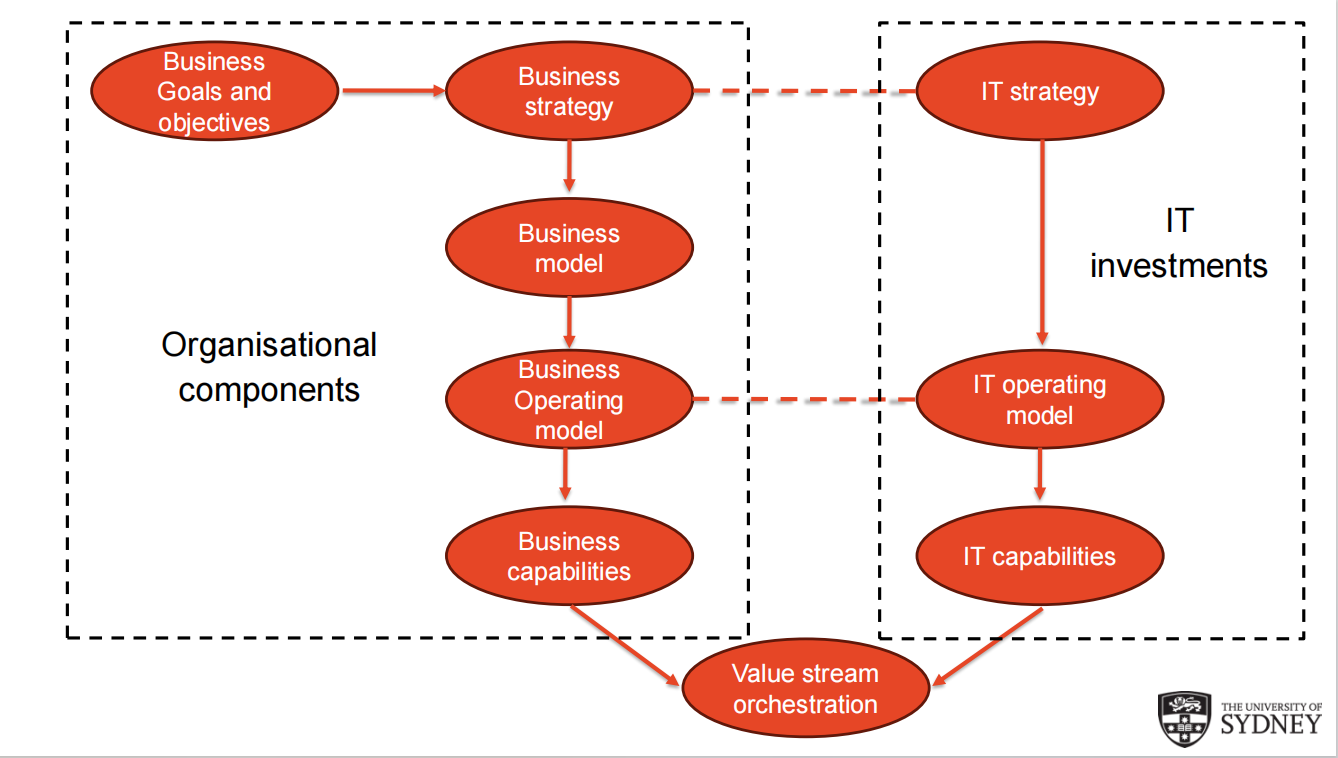
\includegraphics[width=0.8\linewidth]{figures/Week 2/two sides.png}
\end{figure}

\noindent Explanation:

\textbf{Organisation side}: This side outlines how an Organisation builds value through \textbf{business planning and operational structure}: Business goals and objectives, business strategy, business models, business operating models, and business capabilities.

\bigskip

\textbf{IT investment side}: This side shows how IT must align with business to support and enable value creation: IT strategy, IT operating model, and IT capabilities.

\subsubsection{Business goals and objectives}

\indent

Business goals and objectives are the foundation of all Organisational activity. They define the \textbf{vision}, \textbf{mission}, and \textbf{desired outcomes}. These guide both business and IT strategies. They \textbf{define value at the core}, because value begins with a clear understanding of what the Organisation
wants to achieve..

Objectives specify the methods, paths and metrics that can help an Organisation achieve a goal.

\subsubsection{Business goals VS Business objectives}

\indent

Business goals and business objectives are closely related, and the terms are sometimes used interchangeably. However, they are two different things.

\textbf{Business goals} represent the direction in which a company intends to go and 
define what the Organisation wants to achieve. 

\textbf{Business objective} specifies the methods and paths that can help a 
business achieve that goal.

\subsubsection{Business Strategy}

\indent

Business strategy outlines \textbf{how the Organisation will achieve its goals}. This includes choices around target markets, competitive positioning, resource allocations, etc. IT must be aligned with this strategy to be effective.

\textbf{Strategy drives both structure and technology direction.}

\subsubsection{IT strategy}

\indent

IT strategy is the roadmap for \textbf{how technology will support business strategy}. It focuses on digital transformation, infrastructure decisions, innovation plans, etc.

\textbf{IT strategy must be developed in lockstep with business strategy}.

\subsubsection{Business models}

\indent

The business model defines \textbf{how value is created, delivered, and captured}. It can be best show as a Business Model Canvas (BMC). Business models guide IT system requirements (e.g., eCommerce platforms, CRMs).

\textbf{A solid model ensures the strategy is executable.}

\subsubsection{Operating models}

\indent

An operating model is the blueprint for how value will be created and delivered to stakeholders.

It details how an Organisation configures and re-configures (orchestrates) its capabilities to create and deliver value to the Organisation to achieve its goals and strategic objectives.

An operating model also defines how the Organisation manages itself and its resources through its management processes, governance and culture.

Any change to the Organisation’s business models will require changes to the operating model.

\subsubsection{Business operating model}

\indent

The business operating model defines \textbf{how the organisation is structured and operates}. It describes centralization vs decentralization, business units and 
interdependencies, decision making authority, etc. Determines the IT support and governance model required.

\textbf{Operating model alignment enables efficient IT integration}.

\subsubsection{IT operating model}

\indent

Defines \textbf{how IT functions are structured and governed}. This includes IT service delivery, vendor management, project management, agile practices, etc. Must align with the business operating model.

\textbf{Efficient IT operations are critical for smooth execution}.

\subsubsection{Business capabilities}

\indent

Capabilities are the \textbf{skills, processes, and resources} the business uses to deliver value. Examples: logistics, R\&D, customer service, data analytics. Must be supported and often enhanced by IT (e.g., automation, AI, CRM systems).

\textbf{IT enables, enhances, or transforms these core capabilities.}

\subsubsection{IT capabilities}

\indent

IT capabilities refer to the technical strengths of the IT function. For example, system integration, cloud management, data analytics and reporting, cybersecurity, etc. These directly support and scale business capabilities.

\textbf{Strong IT capabilities are essential for digital competitiveness}.

\subsubsection{Value stream orchestration}

\indent

Value stream orchestration is about c\textbf{oordinating business and IT to deliver continuous value}. It involves synchronizing people, processes, and technology to \textbf{maximize the value delivered to stakeholders}. Enables smooth flow of value from idea to delivery.

\textbf{Orchestration ensures technology investments produce real 
business outcomes.}

\subsection{Best practices for IT investments}

\begin{itemize}
    \item Ensure every IT investment supports overall business goals.
    \item Engage business leaders in IT planning.
    \item Set measurable outcomes for each IT investment (e.g., cost savings, process efficiency, customer experience).
    \item Use KPIs to track ROI over time.
    \item Use a cost-benefit or value-risk matrix to rank IT initiatives.
    \item Focus on projects that provide both short-term wins and long-term value.
    \item Invest in technologies that can grow with the business (e.g., cloud, APIs, modular platforms).
    \item Avoid systems that lock the business into rigid structures.
    \item Encourage experimentation with emerging tech (AI, blockchain, IoT) in low risk areas.
    \item Balance innovation with practical business value
\end{itemize}

\subsection{Question}

\subsubsection{End of lecture questions}

\begin{itemize}
    \item Define the term “Organisation” and explain how it differs from a “business”.
    \item What is the difference between value and organisational value? Provide an example to illustrate.
    \item Explain the distinction between resources and capabilities with examples.
    \item List and briefly describe any three types of organisational structures.
    \item What is ‘value stream orchestration’ in the context of IT and business alignment?
\end{itemize}

\subsubsection{Case-study based questions}

\indent 

BrightCare is a mid-sized private healthcare organisation that specializes in telehealth services and digital patient records. The management has identified a need to increase organisational value by improving service delivery, enhancing patient satisfaction, and reducing operational costs. Currently, their systems are outdated, departments are siloed, and reporting is mostly manual.

The company has decided to:

\begin{itemize}
    \item Invest in a new cloud-based health information system (HIS)
    \item Hire a Chief Information Officer (CIO) to align IT strategy with the company’s vision
    \item Restructure from a functional model to a matrix structure to enable cross-departmental collaboration
\end{itemize}

The CIO proposes the following plan:

\begin{itemize}
    \item Define clear business goals (e.g., 30\% reduction in wait times, 95\% digital record accuracy)
    \item Align IT and business strategies by upgrading technology and retraining staff
    \item Build capabilities in data analytics and real-time reporting
    \item Implement value stream orchestration to connect IT workflows with patient care delivery
\end{itemize}

\noindent \textbf{Question}:

\begin{itemize}
    \item Identify two business goals BrightCare is trying to achieve through IT investment. How do these relate to Organisational value?
    \item What kind of Organisational structure was initially in place at BrightCare, and why is the move to a matrix structure beneficial in this context?
    \item Explain the role of the CIO in ensuring alignment between IT and business at BrightCare. What challenges might the CIO face?
    \item Evaluate whether the planned IT investment is likely to create organisational value. Justify your answer using concepts from the lecture.
\end{itemize}